In this Section we describe the methodology that we have followed to deploy a Hadoop cluster instance inside the FedCloud federated cloud infrastructure. Basically, it consists of two processes: 
\begin{enumerate}
\item \emph{Cluster startup}: obtaining the resources necessary to form the cluster from each of the sites in FedCloud and configure the Hadoop cluster
\item \emph{Benchmarks}: loading the data sets and running various MapReduce jobs
\end{enumerate}
Each of these processes is described in more detail in the following subsections.

\subsection{Cluster startup}
\label{ssect-cluster}

A general overview of the overall cluster startup process is given in Figure~\ref{fig:client}.
% VM template & Marketplace
A customized virtual machine (VM) image template that includes all the software necessary was created. This image is based on Scientific Linux 6.4 and contains the following customizations:
\begin{itemize}
\item \emph{Firewall:} iptables is configured to allow only inter-cluster communication except for remote ssh access using public key authentication.
\item \emph{SSH:} enable root access through SSH public key authentication (\emph{authorized\_keys}).
\item \emph{Modules:} we make use of the Modules package to simplify the deployment of the software needed to run Hadoop.
\item \emph{Java:} we used both Oracle Java JDK 1.6 and 1.7
\item \emph{Hadoop:} different versions of Hadoop are included up to 1.2.1 (latest stable version in the v1 branch). The configuration using Modules makes easy to include additional versions and decide the one we want to use when starting the Hadoop cluster.
\end{itemize}


This customized image was registered in the EGI Marketplace~\cite{marketplace} which provides a common place where where we can can store images. Unfortunately, the Marketplace does not store the VM images into a common repository, it just shows which resource providers (RPs) have the VM image available at their endpoint. This means that each RP has to manually download the image to his local site in order to make it available at his endpoint. 

% Client: rOCCI + VOMS
The next step is to instantiate the virtual machines that will form the Hadoop cluster, for this purpose we make use of the new implementation of the OCCI 1.1 specification under rOCCI~\cite{rocci} as well as our VOMS proxy credentials. The new rOCCI implementation provides several advantages like the fact that we are able to avoid the previous issue that all user certificates request are mapped to a single ONE\_USER account.
Additionally, the usage of VOMS over plain X509 auth greatly simplifies the access to the different sites that form FedCloud without the need to request each site to give access to our X509 certificate's DN.

Unfortunately FedCloud does not count with a workload management system, so each VM creation request must be sent to the appropriate endpoint. This means that we have to take care ourselves of the partitioning of the cluster between the different FedCloud sites.

%\begin{figure}[h]
%\centering
%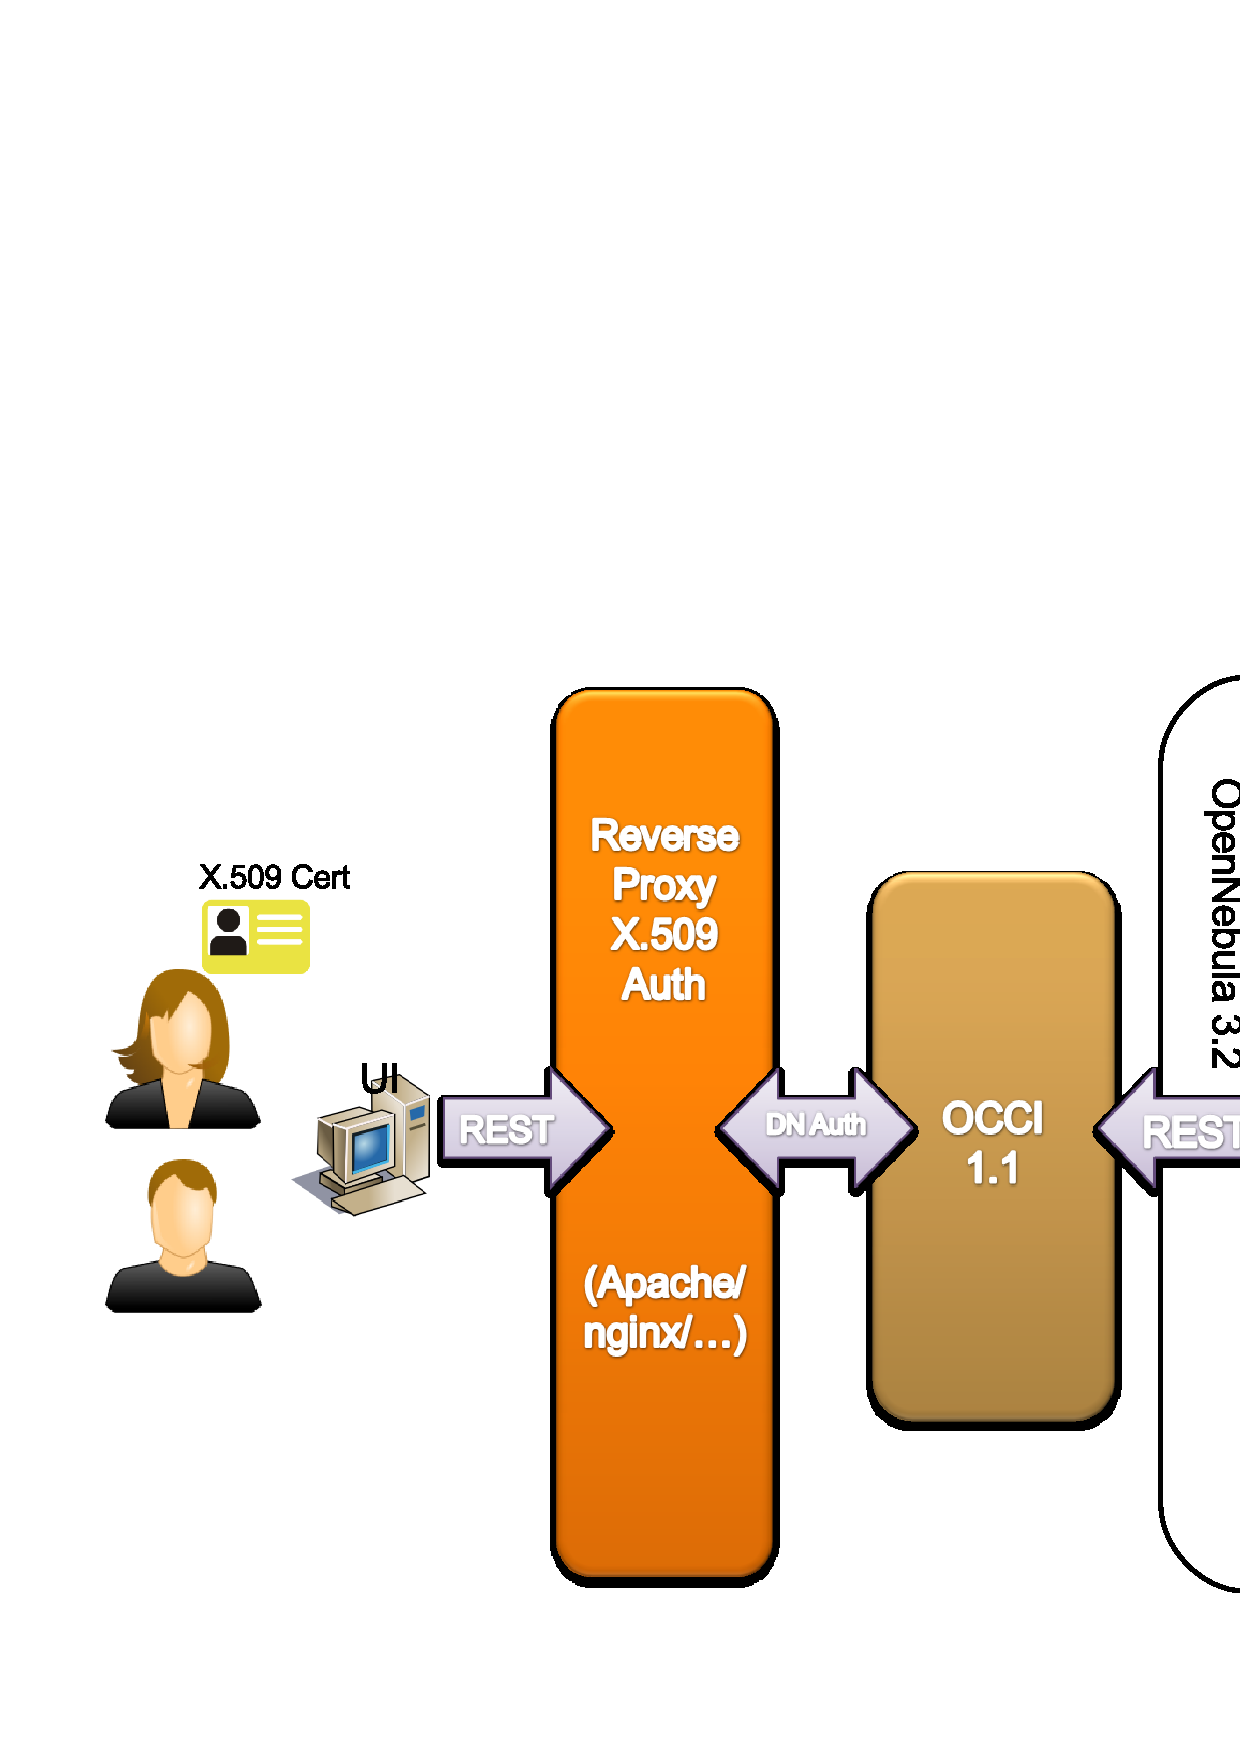
\includegraphics[width=0.8\textwidth]{figures/occi_opennebula.png}
%\caption{OCCI 1.1 server and x509 auth for OpenNebula.}
%\label{fig:occi1}
%\end{figure}

\begin{figure}[h]
\centering
\includegraphics[width=\textwidth]{figures/client-v2.png}
\caption{Cluster startup process using rOCCI and VOMS from a single UI.}
\label{fig:client}
\end{figure}

% Resources used
About the resources used by each of the instances, in order to increase the concurrent number of VMs, we used small size VM instances with 1GB of RAM and 1 CPU for the wordcount benchmarks and 2GB of RAM and 1 core for the TeraGen and TeraSort bechmarks (see Section \ref{ssect-benchmarks}).


% Basics about Hadoop services needed: hadoop-master, slaves
Our Hadoop clusters will consist of one \emph{master} node and a variable number of \emph{slave} nodes depending on the size of the cluster. For example in the case of a 101 node cluster, one node will be configured as master and the remaining 100 as slaves. The master node will run the \emph{namenode}, \emph{secondarynamenode} and \emph{jobtracker} services and each of the slaves will run just one \emph{tasktracker} and one \emph{datanode} services
due to the fact that we are using small VM instances with just 1GB of RAM and 1 CPU we decide to run just one tasktracker and one datanode per slave. 

 The tuned configuration parameters are given in Table \ref{table:conf}. The column type identifies the configuration file where the parameter is set, the complete configuration files can be found at~\cite{scripts}.
% TODO: figure showing the master/slave setup and the services
% Hadoop configuration
%% Hadoop 1.0.3
%% Oracle Java JDK 1.6.0_33
%% Modules

These parameters have been configured to adapt the Hadoop cluster to resources available--1GB of RAM and 1 CPU per node--. The $dfs.replication$ parameter indicates how many copies we want to store of each block, in this case we use three replicas that will allow different nodes to execute the same mapreduce tasks--speculative execution--mitigating the performance degradation that could be experienced in a heterogeneous cluster with VMs running under hypervisors with different load conditions. The $mapred.tasktracker.map.tasks.maximum$ and $reduce.tasks.maximum$ are set to 1 because we only have 1 CPU available to run both services and the HADOOP\_HEAPSIZE is set to 512MB to allow both running at the same time without exhausting the node's memory. The number of reduce tasks, $mapred.reduce.tasks$, is set to 95\% of the number of slaves in the Hadoop cluster. 

As we will see in Section \ref{ssect-execution} our Hadoop installation will cope with two very different use cases that influence our decission about the $dfs.block.size$ values to use. In the case of the Encyclop{\ae}dia Britannica's use case the block size is set to 1MB and in the Wikipedia's use case, that uses a much larger data set, to 64MB. Under this conditions both use cases generate less than 700 total mapreduce tasks which can be handled well by our hadoop master node which has only 1GB of RAM and 1 CPU.


%% table with the parameters used
% TODO: complete the table
\begin{table}[h!]
\caption{Tuned Hadoop configuration for small VM instances. It includes both the HDFS and MapReduce parameters used.}
\label{table:conf}
%
\vspace{-0.5em}
%
\begin{center}
\begin{tabular}{ccc}
\toprule
%Parameter				& Type\tablenotemark[a] & Value	 	\\
Parameter				& Type 			& Value	 	\\
\midrule
$fs.inmemory.size.mb$			& core-site		& 200MB	 	\\
$io.file.buffer.size$                  	& core-site		& 128KB  	\\
$mapreduce.task.io.sort.factor$ 	& core-site		& 100	 	\\
$mapreduce.task.io.sort.mb$ 	 	& core-site		& 100	 	\\
$mapred.tasktracker.map.tasks.maximum$ 	& mapred-site		& 1	 	\\
$mapred.tasktracker.reduce.tasks.maximum$ & mapred-site		& 1	 	\\
$mapred.reduce.tasks$ 			& mapred-site		& $0.95\times$\emph{num.~slaves} \\
$dfs.datanode.du.reserved$ 		& hdfs-site		& 1GB	 	\\
$dfs.block.size$ 			& hdfs-site		& 1MB / 64MB 	\\
$dfs.replication$ 			& hdfs-site		& 3	 	\\
HADOOP\_HEAPSIZE            	 	& hadoop-env   		& 512MB 	\\
%HADOOP\_OPTS                	 	& hadoop-env   		& $-XX:+UseParallelGC$ 	\\
%                             	 	&              		& $-Djava.net.preferIPv4Stack=true$ 	\\
%
%(1,5,0)		& 0.0645	& 0.0689\tablenotemark[d]	& $2 \times 10^{-4}$		\\
%
\bottomrule
\multicolumn{3}{c}{\rule{0.98\textwidth}{0em}}\\
%\rule{0.3\textwidth}{0cm} & \rule{0.2\textwidth}{0cm} &  \\
\end{tabular}
\end{center}
%\vspace{-3.5em}
%\tablenotetext[a] {Identifies the configuration file where the parameter is set, the complete configuration files can be found at \url{https://github.com/grid-admin/hadoop}}
\end{table}


%% TODO: Explain the values of the parameters used


\subsection{Benchmark execution}
\label{ssect-execution}

In order to evaluate the suitability of FedCloud to perform Big Data analytics using Hadoop we selected two use cases which are quite representative of a broad range of jobs that could be performed in a Hadoop cluster. The benchmarks were run both in a federated cluster deployment and in a one-site-only cluster deployment, allowing us to compare the results and analyse the expected degradation when using remotely distributed resources.

% Encyclopaedia Britannica 1911: 176MB
%% -put (5 runs)
%%% Upload from hadoop-master
%% wordcount (5 runs)

% Wikipedia: 41GB
%% -put (1 run)
%%% Upload from UI (hadoop-master does not have enough space to store it)
%% wordcount (5 runs)


The first use case is based in the Encyclop{\ae}dia Britannica\cite{britannica} data set--the 1911 version that is already in the public domain--. This represents a rather small data set of just 176MB, so that this use case can be considered as a small scale benchmark that will serve to evaluate the expected degradation in performance due to fact that we will be using federated resources located at different sites. The data set is downloaded directly from the master node and later on it is distributed from there to the slaves, what is called a \emph{put} operation in Hadoop argon. This use case has a great overload due to the creation of rather small mapreduce tasks that will stress the communication system because it uses a rather small block size of just 1MB, so each map operation has little to process.

The second use case is based in the Wikipedia\cite{wikipedia} data set. This represents a much larger data set comprising 41GB, so it can be considered a more realistic benchmark of a Big Data application. Due to the size of the data set the files could not be downloaded directly in the master node so the \emph{put} operation is done directly from our local Hadoop client located at CESGA. This use case will incur in a lower task creation penalization because it uses a larger block size of 64MB, so each map task will take much longer than the time needed for its creation.


The benchmarks are run for different cluster sizes that range from 10 to 101. In all the benchmarks we measure two parameters:
\begin{enumerate}
\item \emph{The put time:} the time to load the files into the Hadoop HDFS filesystem 
\item \emph{The wordcount time:} the time to perform a simple wordcount mapreduce job that computes the number of occurrences of each word over the complete data set. 
\end{enumerate}
All the measurements where repeated at least 5 times in order to evaluate the variability of the results, the only exception were the \emph{put} times for the Wikipedia that due to its duration could only be run once.


